\documentclass[11pt]{article}
\usepackage[margin=1in]{geometry} 
\usepackage{hyperref} 
\usepackage{lastpage}
\usepackage{fancyhdr}
\usepackage{csvsimple,booktabs}
\usepackage{graphicx}
\pagestyle{fancy}
\setlength{\headheight}{42pt}
\usepackage{times}

\begin{document}
\lhead{Ingeniería Física \\ Escuela de Física \\ Tecnológico de Costa Rica} 
\rhead{Instrumentación I \\ Tarea \#2  \\ Entrega: Semana 6} 
\cfoot{\thepage\ de \pageref{LastPage}}
\setlength{\parindent}{0em}

\textbf{Diseño de un sistema de medición de temperatura por globo conforme a la norma ISO 7243}

\section*{1. Contexto y justificación}
La medición de temperatura por globo se utiliza para determinar la carga térmica radiante a la que está expuesta una persona y forma parte del cálculo del índice \href{https://www.youtube.com/watch?v=EIJeJcLun7Y}{\textbf{WBGT}} (\textit{Wet Bulb Globe Temperature}), definido en la norma \textbf{ISO 7243}. Este índice permite evaluar el \textbf{estrés térmico} en ambientes cálidos combinando diferentes parámetros:

\begin{itemize}
    \item \textbf{Temperatura del aire} ($t_a$)
    \item \textbf{Temperatura de bulbo húmedo natural} ($t_{nw}$)
    \item \textbf{Temperatura de globo negro} ($t_g$)
\end{itemize}

En esta tarea, se requiere \textbf{diseñar un sensor de temperatura de globo}. Para ello, se utilizará un \textbf{sensor de temperatura convencional} que se instalará dentro de un \textbf{globo negro} con las dimensiones, emisividad y características especificadas por la \textbf{ISO 7243}. A este conjunto se le denomina \textit{sensor de temperatura de globo}.  

Además, deberá elaborar un \textbf{diagrama de conexiones eléctricas} conforme a la norma \textbf{ANSI ISA 315 - 2009} y proponer una \textbf{representación gráfica} del montaje del sistema.

\section*{2. Objetivos de la tarea}
\begin{itemize}
    \item \textbf{Diseñar} un sensor de temperatura de globo que cumpla con las especificaciones de la norma ISO 7243, integrando un sensor de temperatura convencional dentro de un globo negro.
    \item \textbf{Diseñar} un diagrama de conexiones del sistema completo utilizando la simbología eléctrica estandarizada (ANSI ISA 315-2009).
    \item \textbf{Proponer} una representación gráfica detallada de cómo se vería el sistema montado, incluyendo el sensor, el globo y los elementos de instrumentación.
\end{itemize}

\section*{3. Diseño del sensor de temperatura de globo}
Consultar la norma \href{https://es.slideshare.net/slideshow/international-standard-iso-7243/251054896}{ISO 7243} y determinar qué características mínimas debe cumplir el sensor que se instalará dentro del globo negro.  
El objetivo es diseñar un sensor de temperatura de globo funcional, integrando correctamente los elementos necesarios.

Para guiar el diseño, considere las siguientes \textbf{tres preguntas clave}:

\begin{enumerate}
    \item \textbf{Rango de medición y precisión:} \\
    ¿Cuál es el rango de temperatura y la tolerancia mínima que debe cumplir el sensor convencional para garantizar mediciones confiables en conjunto con el globo? (Ver Anexo B, sección B.2).
    \item \textbf{Dimensiones y material del globo:} \\
    ¿Por qué es importante que el globo tenga un diámetro de \textbf{150\,mm}, un coeficiente de emisión de \textbf{0,95} y un espesor del material lo más delgado posible? (Ver Anexo B, sección B.2).
    \item \textbf{Tiempo de respuesta y montaje:} \\
    ¿Qué consideraciones deben tomarse en cuenta para evitar errores por blindaje involuntario del globo y asegurar que el sensor registre una temperatura estable? (Ver Anexo B, sección B.2).
\end{enumerate}

\section*{4. Diagrama de conexiones}
Usando el estándar \href{https://www.scribd.com/document/621156343/ANSI-ISA-5-1-2009-Traducido}{ANSI/ISA-315-2009}, realice un diagrama que describa de mejor manera el proceso de medición descrito. Un ejemplo de un diagrama base sería el de la figura \ref{ejemplo 2}.
\begin{figure}[h]
    \centering
    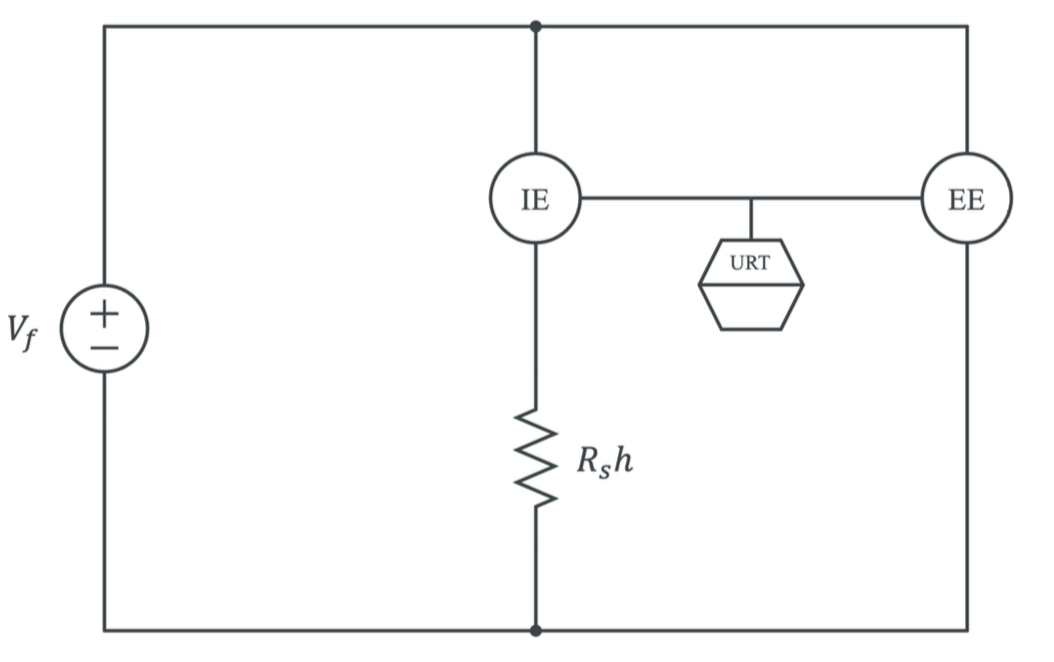
\includegraphics[width=0.4\linewidth]{fig/diagrama2.jpg}
    \caption{Medición de corriente y voltaje en un circuito}
    \label{ejemplo 2}
\end{figure}

Este diagrama debe mostrar:

\begin{itemize}
    \item Sensor de temperatura convencional instalado dentro del globo.
    \item Microcontrolador o dispositivo de adquisición de datos.
    \item Fuente de alimentación.
    \item Líneas de conexión, indicando señales analógicas, digitales y de referencia.
\end{itemize}

El objetivo es que el diagrama represente \textbf{todas las interconexiones del sistema}, asegurando que otro estudiante pueda replicar el diseño únicamente con base en el plano.

\section*{5. Representación gráfica del sistema}
Realice de manera gráfica el sistema. Para esto se debe incluir el circuito donde estén las conexiones y el sensor, además de cómo se conecta el sistema para medir la temperatura del globo. Puede presentarlo como un dibujo o esquema detallado. 

Tomar en cuenta los siguientes aspectos:
\begin{itemize}
    \item La posición del globo negro con el sensor en su interior.
    \item El soporte o estructura donde se instala el globo.
    \item Los cables de conexión hacia el sistema de adquisición de datos.
    \item Una leyenda que identifique cada componente.
\end{itemize}

Este esquema debe reflejar la integración física de todos los elementos y servir como referencia para el montaje real.

\end{document}
